	\begin{tabular}{ | c   p{18cm} |}
		\hline
		\cellcolor{black}\rotcell{\large\textbf{\textcolor{white}{Kondensator}}}  &
		\setlength{\extrarowheight}{10pt}	
		
		\begin{tabular}{L{5cm} L{6.5cm} L{5.3cm}}
			
			\rowcolor[rgb]{1,1,1}
			\textbf{Kapazität}&$\displaystyle C = \frac{Q}{U}$&$\displaystyle[C]= F=\frac{C}{V}$\\[5pt]
			
			
			\rowcolor[rgb]{0.91,0.91,0.91}
			\textbf{Plattenkondensator}& $	{\displaystyle C=\varepsilon _{0}\varepsilon _{\mathrm {r} }\cdot {\frac {A}{d}}}$\qquad$\displaystyle E={\frac {Q}{\varepsilon _{0}\varepsilon _{\mathrm {r} }A}}$   &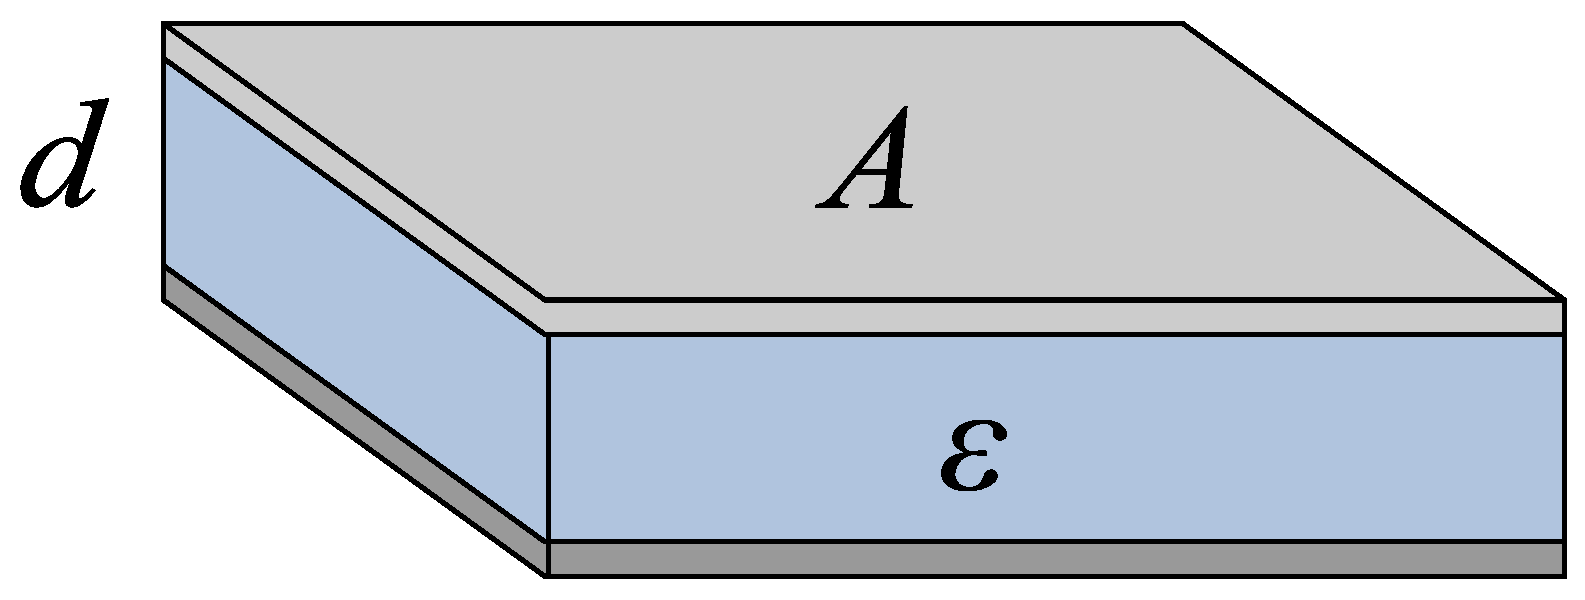
\includegraphics[width=4cm]{platten.pdf}\\
			
			
			
			\rowcolor[rgb]{1,1,1}
			\textbf{Zylinderkondensator}& $	{\displaystyle C=2\pi \varepsilon _{0}\varepsilon _{\mathrm {r} }{\frac {l}{\ln \left({\frac {R_{2}}{R_{1}}}\right)}}}$ \quad $\displaystyle E(r)={\frac {Q}{2\pi rl\varepsilon _{0}\varepsilon _{\mathrm {r} }}}$ &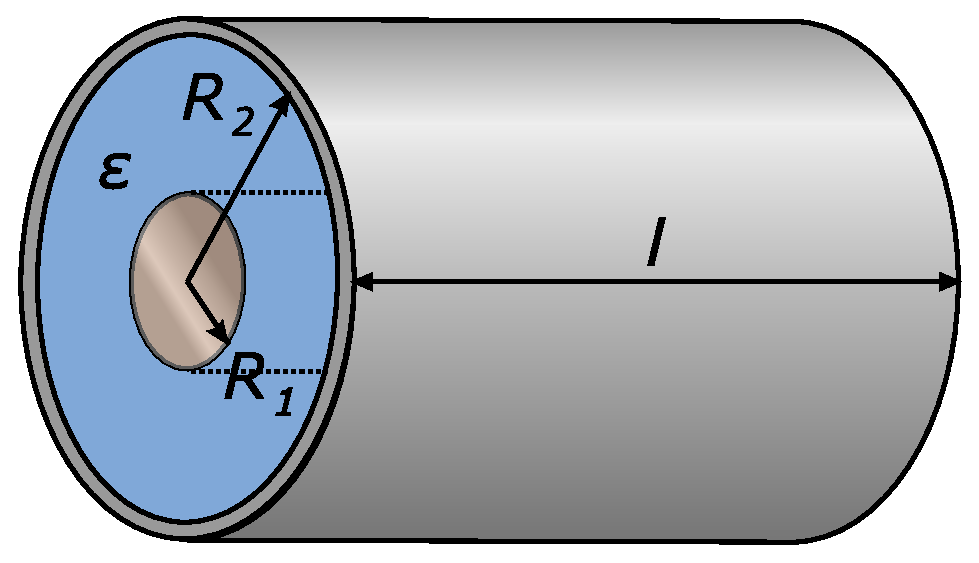
\includegraphics[width=3.5cm]{zylinder.pdf}\\
			
			
			\rowcolor[rgb]{0.91,0.91,0.91}
			\textbf{Plattenkondensator}& $	\displaystyle C=4\pi \varepsilon _{0}\varepsilon _{\mathrm {r} }\left({\frac {1}{R_{1}}}-{\frac {1}{R_{2}}}\right)^{-1}$  \quad
				$\displaystyle E(r)={\frac {Q}{4\pi r^{2}\varepsilon _{0}\varepsilon _{\mathrm {r} }}}$
				 &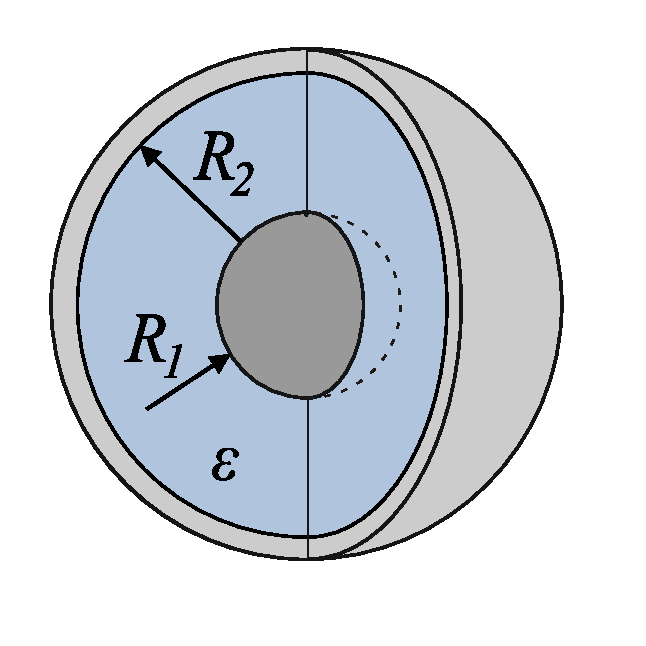
\includegraphics[width=3cm]{kugel.pdf}\\
				 
				 
				 
			\rowcolor[rgb]{1,1,1}
			\textbf{Gespeicherte Energie} \qquad einer Kapazität&	 
			$\displaystyle W_e = \frac{Q^2}{2C} = \frac{CU^2}{2} = \frac{QU}{2}	$ & $\displaystyle [W_e]=J =Ws$
			\\
			
			\rowcolor[rgb]{0.91,0.91,0.91}
			\textbf{Energiedichte} \qquad\qquad\qquad eines Elektrischen Feldes&	 
			$\displaystyle w_e = \frac{\delta W_e}{\delta v} = \frac{1}{2}\vec{D}\cdot \vec{E} = \frac{1}{2}\epsilon E^2	$ & $\displaystyle [w_e]=\frac{J}{m^3} =\frac{Ws}{m^3}$
			\\[5pt]
			
			\rowcolor[rgb]{1,1,1}
			\textbf{Serie / Parallelschaltung}&	 
			$\displaystyle \frac{1}{C}=\sum_{i=1}^{n}\frac{1}{C_i }	$\qquad resp. \qquad$\displaystyle C=\sum_{i=1}^{n}C_i	$ & \\[5pt]
			
			\rowcolor[rgb]{0.91,0.91,0.91}
			\textbf{DGL Kondensator} & $\displaystyle \frac{\delta u_c}{\delta t}= \frac{i_c}{C}$&\\[5pt]
			
			 \rowcolor[rgb]{1,1,1}
			 \textbf{Lade / Entladestrom} Kondensator&	 
			 $\displaystyle I_L (t)= \frac{U_0}{R}\exp^{-\frac{t}{RC}}=-I_E (t)$ & $\tau = RC$ mit $5\tau$ lade/entlade Zeit \\[5pt]
		
		\end{tabular}\\
		\hline
	\end{tabular}